\section{Introduction}\label{sec:intro}

Unlike program verifiers, tools based on symbolic execution~\cite{CD11,DFLO19}
or property-based testing~\cite{CH00,QuickStrom,BeginnerLuck,HC+24} frameworks
\emph{underapproximate} a program's behavior, guaranteeing no false
positives (i.e., every reported bug is a real bug), but admitting
false negatives (i.e., not all real bugs may be reported).  To help
place such tools on a formal footing, new program logics have been
recently proposed~\cite{casl,OHP19,LR+22,ZDS23} that allow reasoning over
\emph{incorrectness} properties of a program.  For example,
incorrectness triples of the form, $[P]\texttt{c}[Q]$ proposed by
O'Hearn~\cite{OHP19} assert that for any post-state of a command
\texttt{c} satisfying assertion $Q$ there must exist a pre-state
satisfying $P$.  This interpretation defines an underapproximation of
\texttt{c}'s behavior because it requires producing a witness
pre-state to justify every valid post-state assertion.

While these proposals define underapproximate axiomatic proof rules
for imperative first-order state-based specifications, there have also
been contemporary efforts that integrate notions of incorrectness and
underapproximation into a type system~\cite{RW24,WGJ24,ZMD+23}.  For example,
~\cite{RW24}  introduces a two-sided type system that allows for the
refutation of typing formulas, guaranteeing that not only do
well-typed programs not go wrong, but also that ill-typed programs
don't evaluate; ~\cite{ZMD+23}  leverages notions of underapproximation
in the form of \emph{coverage} types to represent the set of values
guaranteed to be produced by a test generator.

These type systems provide compositional reasoning about
underapproximations in a purely functional setting, but cannot be
directly applied to impure functional programs, for example those that
interact with effectful libraries.  To address this important
limitation, this paper introduces \tyName{}, \emph{Underapproximate
  Hoare Automata Types}, a type abstraction for \emph{underapproximate
  effectful computations}.  A \tyName{} type judgement takes the form:
\[\vdash e\, :\, [H]\,t\,[F]\]
\noindent where $H$ and $F$ qualify type $t$ with pre- ($H$) and post-
($F$) conditions.  In our setting, these conditions are expressed
using the language of symbolic regular expressions (SREs), an
algebraic representation of the symbolic finite automata used
in~\cite{ZYDJ24}, to specify effect traces.  Unlike the overapproximate
interpretation given for \textsc{hat}s in earlier work, however, a
\tyName{} expresses underapproximate behavior: the judgement above
states that for every possible sequence of effect traces $F$
producible by $e$ and consistent with type $t$, there exists an effect
trace accepted by $H$.  Intuitively, a \tyName{} expresses the
conditions (i.e., $H$) that \emph{must} hold prior to executing an
expression $e$ to guarantee the effects it produces (i.e., $F$) are
realizable.

To illustrate, the following \tyName{} captures the underapproximate
behavior that constrains the set of values visible to a $\eff{get}$
operation in the context of previously executed $\eff{put}$s in a
setting where a program interacts with a key-value store using these
operations:
\begin{align*}
  \eff{get}: x{:}\Code{Value.t} \garr k{:}\Code{Key.t} \sarr \effLR{\allA\ \msgA{put}{k\;x}\ \allA }
  \{\vnu:\Code{Value.t}\,|\,\vnu = x\} \effLR{\msgA{get}{k\; x}}
\end{align*}
This \tyName{} asserts that a $\eff{get}$ operation is guaranteed to
produce a trace consisting of a single effect, $\msgA{get}{k\; x}$,
provided that some $\eff{put}$ operation binding $k$ to $x$ ($\allA
\msgA{put}{k\;x} \allA$) was executed before. (Here, $x$ is a ghost
variable used to capture the dependence between a $\eff{put}$
operation that stores a value and a subsequent $\eff{get}$ that reads
that value.)  The underapproximation interpretation of \tyName{}
encodes a form of reachability and data dependence - the execution of
a $\eff{get}$ operation on a key $k$ is dependent on the execution of
a previous $\eff{put}$ operation on $k$.

In this paper, we use \tyName{}s as a specification mechanism to guide
a property-based test (PBT) generation synthesis procedure.  PBT has
become an increasingly popular framework that allows automated testing
of user-specified properties.  Generators that produce input values to
the system-under-test (SUT) are a central component of a PBT system,
but manually writing generators is a well-known pain point~\cite{HC+24}
to their wider adoption.  To be effective, a generator should only
produce inputs that satisfy the SUT's precondition because input that
don't are simply discarded.  While generators can be automatically
derived for inputs that have simple types, writing generators for SUTs
whose inputs have deep structural or semantic constraints remains a
publication-worthy exercise~\cite{pbt-ifc,PCRH+11,BeginnerLuck,FQL24}.

The challenges with writing PBT generators are further exacerbated
when the SUT is effectful.  In this setting, tests are typically
comprised of \emph{sequences} of inputs that induce effects in a
particular order to expose latent data and control dependencies
relevant to the property being checked.  Examples of applications
in which tests are naturally crafted in this fashion include:
\begin{enumerate}

\item \textbf{Library API invocations:} The SUT is a library
  implementing an effectful abstract data type (ADT) with a set of
  APIs.  A test consists of a sequence of API calls that are
  expected to lead the implementation to an error state (e.g., a
  violation of a representation invariant~\cite{MP+20,ZYDJ24}).

\item \textbf{Serialized inputs:} The SUT is a procedure that
  processes serialized input data, reconstructs an AST from this
  input, and operates over the resulting structure.  The inputs
  produced by the test generator are expected to establish semantic
  dependencies among nodes in the corresponding AST that do not
  satisfy a property of interest (e.g., evaluation errors due to
  incorrect treatment of variable scoping or binding).

\item \textbf{Database transactions:} The SUT is a database supporting
  transactional read and write operations under various isolation
  levels.  A test consists of a sequence of transaction operations
  whose interleaved order is chosen to expose violations of isolation
  or consistency guarantees the database is supposed to provide.

\item \textbf{Distributed protocols:} The SUT is a distributed system
  whose components are expected to adhere to protocol invariants.  A
  test is a sequence of message invocations that lead the system to a
  global state in which these invariants are not maintained.
\end{enumerate}
A common feature shared by these examples, despite being drawn from
diverse domains, is the requirement that the test generator be
cognizant of how event dependencies are (or are not) meaningful to
manifesting a property violation.  To capture this information
succintly, we use \tyName{}s as a formal specification language to
precisely describe latent dependencies among effectful operations, and
expose these dependencies in a domain-specific language tailored for
writing generators that produce sequences conforming to these
dependencies.  For the specification given above, a well-typed program
written in our DSL would only generate test sequences in which every
$\eff{get}$ operation is proceeded by at least one $\eff{put}$ on the
same key, with no other constraints on operations that might be
interspersed between them.  While \tyName{}s used in this way help
check that a generator is effective, the burden of writing the
generator still remains.  To alleviate this overhead, we connect these
two elements by defining a program synthesis technique to
automatically construct DSL generator programs from \tyName{}
specifications.

Figure~\ref{fig:workflow} depicts the workflow of our system, named
\name.  Relevant APIs of the SUT are specified using \tyName{}s.
These specifications, along with the property of interest, are
type-checked.  If type-checking is successful, these inputs then drive
the \name{} synthesis procedure which yields a test generator that can
be transpiled into different target languages; thus far, we have
implemented OCaml and P targets.  The test generator program is
guaranteed to produce tests that respect the underapproximate
interpretation of input \tyName{} specifications.
\begin{wrapfigure}{l}{.65\textwidth}
  \centering
  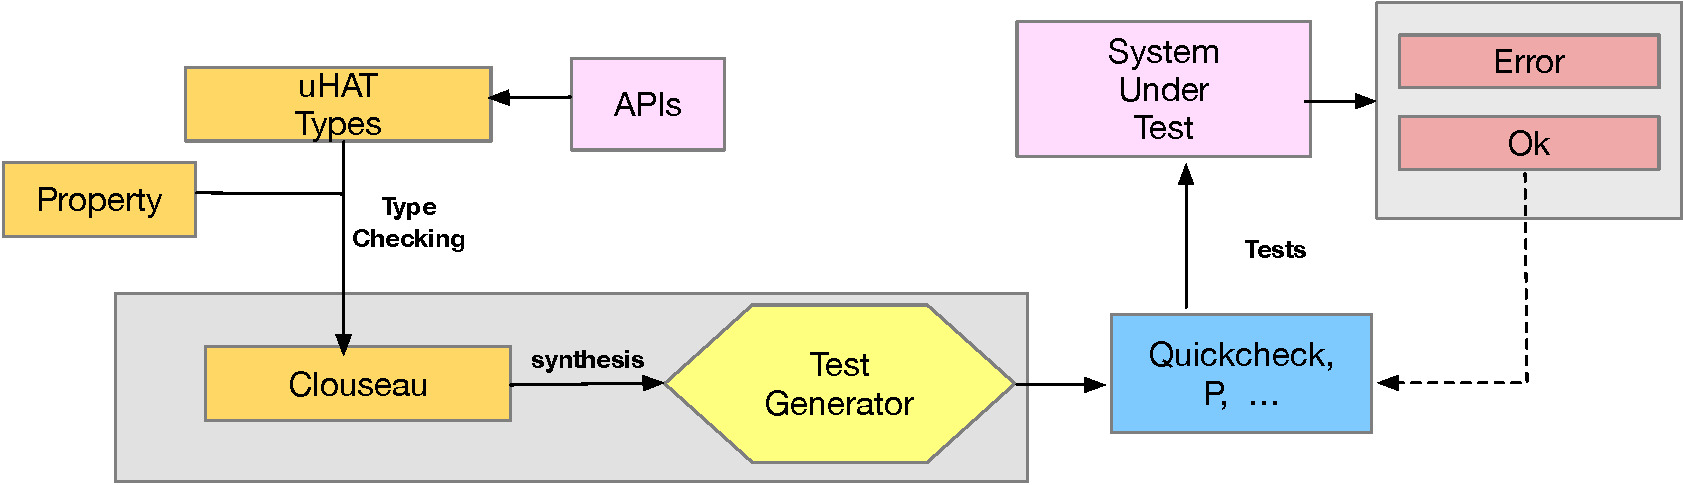
\includegraphics[width=0.98\linewidth]{figures/workflow.pdf}
  \caption{\name\ workflow.}
  \label{fig:workflow}
\end{wrapfigure}
The rest of the paper is organized as follows. In
Section~\ref{sec:overview}, we provide additional motivation for the
problem along with a series of examples to illustrate our approach.
Section~\ref{sec:formal} presents the operational semantics and type
system for our DSL that exposes the underapproximate structure of
\tyName{}s.  The synthesis algorithm that translates these types into
\name{} programs is given in Section~\ref{sec:synthesis}.  We provide
a detailed evaluation over a broad range of diverse benchmarks drawn
from the domains given above to demonstrate the utility of our
approach; these include generating tests for semantically complex data
structure properties such as well-typed simply-typed lambda calculus
terms using de Brujin indices, as well as real-world distibuted
protocols deployed in industry.  Secs.~\ref{sec:related}
and~\ref{sec:conc} present related work and conclusions.

